\documentclass{article}
\usepackage[utf8]{inputenc}
\usepackage[a4paper, total={6.5in, 9in}]{geometry}
\usepackage{fancyhdr}
\usepackage{amsmath, amsthm, amsfonts, mathrsfs}
\usepackage{xcolor}
\usepackage{mathtools, float, subfig}
\renewcommand{\labelenumi}{(\alph{enumi})}

\setlength{\headsep}{4em}
\pagestyle{fancy}
\setlength{\parindent}{0cm}
\setlength{\parskip}{1em}

% ASSIGNMENT INFORMATION
\newcommand{\class}{CS 671}
\newcommand{\hwnumber}{3}

\lhead{Braden Hoagland (bch29)}
\chead{{\class} - HW {\hwnumber}}
\rhead{\today}

\begin{document}

%%%%%%%%%%%%%%%%%%%%
% Statistical Learning: Hoeffding’s Inequality
%%%%%%%%%%%%%%%%%%%%

\section{Statistical Learning: Hoeffding’s Inequality}

\begin{enumerate}
	\item For random variable $X$, Markov's inequality states
		\[
			\mathbb{P}(X\geq a) \leq \frac{\mathbb{E}[X]}{a} .
		\] 
		for $a > 0$. Let $\lambda \geq 0$, then we have
		\begin{align*}
			\mathbb{P}(X \geq \mu_X + t) &= \mathbb{P}(X-\mu_x \geq t) \\
						     &= \mathbb{P}(e^{\lambda(X-\mu_X)}\geq e^{\lambda t}) \\
						     &\leq \frac{\mathbb{E}[e^{\lambda(X-\mu_X)}]}{e^{\lambda t}} && \text{(by Markov's inequality, since $e^{\lambda t}>0$)} \\
						     &= M_{X-\mu_X}(\lambda) e^{-\lambda t}.
		\end{align*}
		Since this holds for all $\lambda \geq 0$, it certainly holds for the minimizing value of $\lambda$, i.e.
		\[
			\mathbb{P}(X \geq \mu_X + t) \leq \min_{\lambda \geq 0} M_{X-\mu_X}(\lambda) e^{-\lambda t}.
		\] 
	
	\item 
		Let $X = \sum_{i=1}^{n} (X_i - \mu_{X_i})$, then by linearity of expectation, its mean is $\mu_X = \sum_{i=1}^n (\mu_{X_i} - \mu_{X_i}) = 0$. The problem then becomes
		\begin{align*}
			\mathbb{P}\left(\frac{1}{n} \sum_{i=1}^n(X_i-\mu_{X_i}) \geq t \right) &= \mathbb{P}\left( X \geq nt \right).
			\intertext{Since $\mu_X = 0$, this is in the form of part $(a)$, so we can apply the Chernoff bound to get}
										 &\leq \min_{\lambda \geq 0} \mathbb{E} \left[ e^{\lambda(X - \mu_X)} \right] e^{-\lambda nt} \\
										 &= \min_{\lambda\geq 0} \mathbb{E} \left[ e^{\lambda \sum_{i=1}^n (X_i - \mu_{X_i})} \right] e^{-\lambda nt} \\
										 &= \min_{\lambda\geq 0} \mathbb{E} \left[ \prod_{i=1}^n e^{\lambda (X_i - \mu_{X_i})} \right] e^{-\lambda nt}.
										 \intertext{Since each $X_i$ is independent, we can move the expectation inside the product to get}
										 &= \min_{\lambda\geq 0} \prod_{i=1}^n \mathbb{E}\left[ e^{\lambda (X_i - \mu_{X_i})} \right] e^{-\lambda nt}.
										 \intertext{Since each $X_i$ lies in $[a,b]$, we then apply Hoeffding's lemma to get}
										 &\leq \min_{\lambda \geq 0} \prod_{i=1}^n \exp \left( \frac{\lambda^2 (b-a)^2}{8}  \right) e^{-\lambda nt} \\
										&= \min_{\lambda \geq 0} \exp \left( \frac{\lambda^2 n (b-a)^2}{8} - \lambda nt \right).
		\end{align*}
		We can set the derivative with respect to $\lambda$ of this expression to 0 to find candidates for optimal $\lambda$.
		\begin{align*}
			\frac{\partial }{\partial \lambda} \exp \left( \frac{\lambda^2 n (b-a)^2}{8} -\lambda nt \right) &= 0 \\
			\exp \left( \frac{\lambda^2 n (b-a)^2}{8} -\lambda nt \right) \left( \frac{\lambda n(b-a)^2}{4} -nt \right)&= 0. \\
			\intertext{Since an exponential can never equal 0, we must have}
			\frac{\lambda n(b-a)^2}{4} -nt &= 0 \\
			\lambda &= \frac{4 t }{(b-a)^2} .
		\end{align*}
		Note that when $t \geq 0$, $\lambda \geq 0$ as well, so it satisfies our constraint. Plugging this into our derived inequality, we have
		\[
			\mathbb{P}\left(\frac{1}{n} \sum_{i=1}^n(X-\mu_{X_i}) \geq t \right) \leq \text{exp} \left( -\frac{2nt^2}{(b-a)^2}  \right)
		\] 
		for all $t \geq 0$.


		\item Let $X$ be either 0 or 10 with equal probability, then for $n=1$, Hoeffding's inequality states
			\[
				\mathbb{P}(X-5 \geq t) \leq \text{exp}\left( -\frac{t^2}{50}  \right)
			\] for all $t \geq 0$. However, we can manually calculate this probability to be
			\begin{align*}
				\mathbb{P}(X-5 \geq t) &= \mathbb{P}(X-5\geq t \;|\; X=0)\mathbb{P}(X=0)  + \mathbb{P}(X-5 \geq t \;|\; X=10)\mathbb{P}(X=10)  \\
							 &= \frac{\mathbb{P}(t \leq -5)}{2} + \frac{\mathbb{P}(t \leq 5)}{2}.
			\end{align*}
			Since $t \geq 0$, the first fraction is always 0, so this becomes
			\[
			\mathbb{P}(X-5 \geq t) =
			\begin{cases}
				0 & t > 5 \\
				1/2 & t \leq 5
			\end{cases}
			\] 
			The difference between the Hoeffding bound and the true probability is shown below as $t$ is varied from 0 to 10.
			\begin{figure}[H]
				\centering
				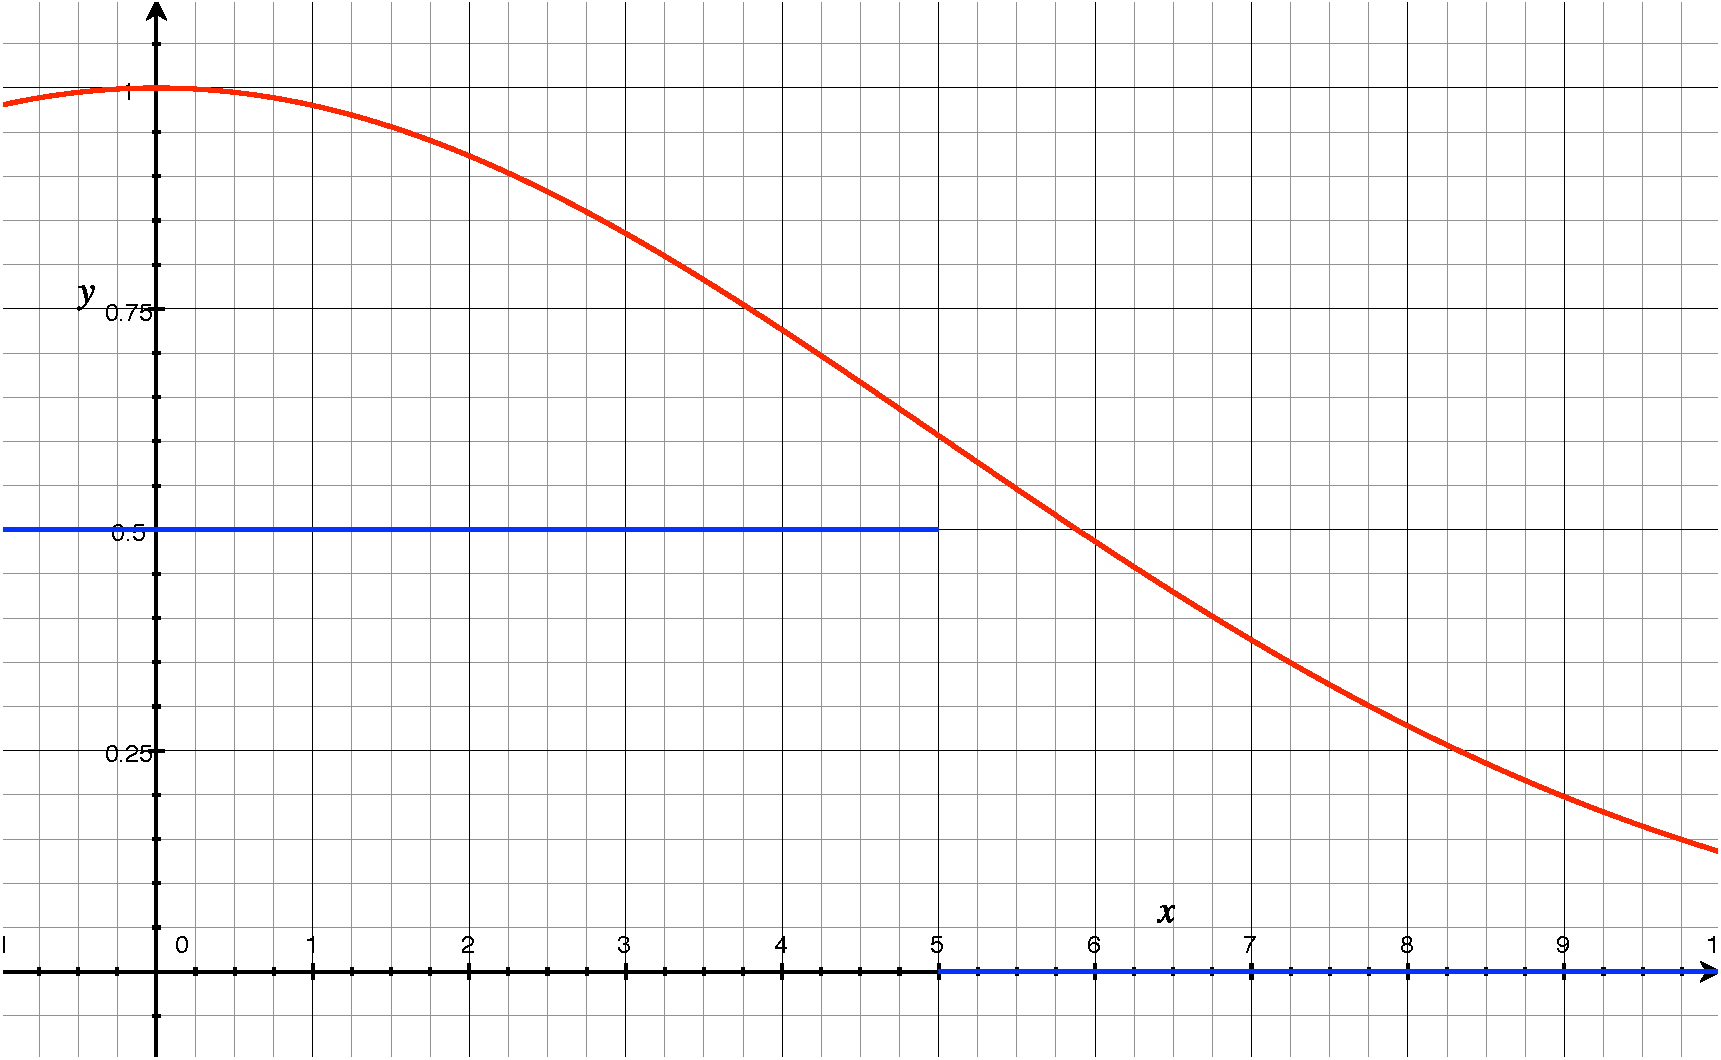
\includegraphics[scale=0.4]{fig/hoeffding.pdf}
				\caption{The Hoeffding bound in red, and the true probability in blue. The $x$-axis represents the value of $t$.}
			\end{figure}
\end{enumerate}


%%%%%%%%%%%%%%%%%%%%
% SVM and the Power of Kernels
%%%%%%%%%%%%%%%%%%%%

\section{SVM and the Power of Kernels}

\begin{enumerate}
	\item The form of the SVM classifier with RBF kernel is
		\begin{align*}
			f(x) &= \sum_{i=1}^n \alpha_i y_i k(x_i,x) + b \\
			     &= \sum_{i=1}^n \alpha_i y_i \exp\left( -\frac{\Vert{x-x_i}\Vert_{\ell_2}^2}{\sigma^2}  \right) + b.
		\end{align*}
		Let $b=0$ and let $\alpha_i=1$ for all $i$, then the classifier becomes
		\[
			f(x) = \sum_{i=1}^n y_i \exp\left( -\frac{\Vert{x-x_i}\Vert_{\ell_2}^2}{\sigma^2}  \right).
		\] 
		If $x=x_i$, then $\exp(-\Vert{x-x_i}\Vert_{\ell_2}^2 / \sigma^2) = \exp(0) = 1$. This means we can rewrite our classifier as
		\[
			f(x_j) = y_j + \sum_{i \neq j} y_i \exp\left( -\frac{\Vert{x_j-x_i}\Vert_{\ell_2}^2}{\sigma^2}  \right).
		\] 
		In the limit as $\sigma\to 0$, every term in the summation becomes 0, so
		\[
			\lim_{\sigma \to 0} f(x_j) = y_j.
		\] Since there are no conflicting labels, this is well defined. Thus this is a valid classifier with 0 training error.

	% 2b
	\item 
		\begin{enumerate}
			\item[(i)]
		Since the data is separable, the optimal decision boundary lies between $a$ and $b$. If the margin is maximized, then the closest points to the decision boundary will be $a$ and $b$. Thus the only support vectors are $a$ and $b$. Thus the dual variable $\alpha_i$ will be 0 if $x_i \neq a$ and $x_i \neq b$.

		The dual problem is then $\max_\alpha \mathcal{D}(\alpha)$, where $\mathcal{D}(\alpha)$ is
		\begin{align*}
			\mathcal{D(\alpha)} &= \sum_{i=1}^{n} \alpha_i - \frac{1}{2} \sum_{i,k} \alpha_i \alpha_k y_i y_k x_i x_j \\
			&= \alpha_a + \alpha_b - \frac{1}{2} \left( 2 \alpha_a \alpha_b y_a y_b x_a x_b + \alpha_a^2 y_a^2 x_a^2 + a_b^2 y_b^2 x_b^2 \right) \\
					    &= \alpha_a + \alpha_b - \frac{1}{2} \left( -2 \alpha_a \alpha_b a b + \alpha_a^2 a^2 + \alpha_b^2 b^2 \right) \\
					    &= \alpha_a + \alpha_b - \frac{1}{2} \left( \alpha_b b - \alpha_a a \right)^2,
		\end{align*}
		such that $\alpha_i \geq 0$ and $\sum_{i} \alpha_i y_i = 0$. Note that since $y_a = 1$ and $y_b=-1$, the second constraint can be rewritten
		\begin{align*}
			\alpha_a y_a + \alpha_b y_b &= 0 \\
			\alpha_a &= \alpha_b.
		\end{align*}
		Thus the dual variable for our two support vectors is the same. Denote this shared value $\alpha_a = \alpha_b$ by $\beta$, then our final statement of the dual problem is
		\[
			\max_\beta \mathcal{D}(\beta) = 2\beta - \frac{1}{2} \beta^2 (b-a)^2
		\] such that $\alpha \geq 0$.

		We can find the optimal $\beta^*$ by setting the derivative of this expression equal to 0 and then solving.
		\begin{align*}
			\frac{d }{d \beta} \mathcal{D}(\beta) = 2 - \beta(b-a)^2 &= 0 \\
			\beta &= \frac{2}{(b-a)^2},
		\end{align*}
		so $\alpha_i^* = 2/(b-a)^2$ if $x_i = a$ or $x_i = b$ and $\alpha^* = 0$ otherwise. Note that $\beta_i^*$ is always non-negative for all $i$ so long as $a$ and $b$ are distinct.

		With the optimal dual variables, we can solve for the classifier $f(x)$. We have
		\begin{align*}
			\lambda^* &= \sum_{i} \alpha_i^* y_i x_i \\
				  &= \alpha_a y_a x_a + \alpha_b y_b x_b \\
				  &= \alpha(b-a) \\
				  &= 2/(b-a)
		\end{align*}
		and
		\begin{align*}
			\lambda_0^* &= 1- \lambda^* x_+ \\
				    &= 1 - \frac{2}{b-a} a,
		\end{align*}
		so the optimal classifier is
		\begin{align*}
			f(x) &= \lambda_0^* + \lambda^* x \\
			     &= 1 - \frac{2}{b-a} a + \frac{2}{b-a} x \\
			     &= 1 - \frac{2}{b-a} (x-a).
		\end{align*}

	\item[(ii)]
		The decision boundary lies at the point $x$ satisfying $f(x)=0$, so we can solve for $x$ to get
		\begin{align*}
			f(x) &= 0 \\
			1 - \frac{2}{b-a} (x-a) &= 0 \\
			x &= \frac{b-a}{2} +a.
		\end{align*}
		This shows that the decision boundary is the midpoint between $a$ and $b$.

	\item[(iii)]
		The number of support vectors can never be 1. Consider the case when there is only one support vector, then all the data lies on one side of the decision boundary, i.e. all points are classified the same. Unless the data is composed of only one class, this will produce large errors for all misclassified points. Thus the optimal classifier for any non-trivial dataset cannot have only 1 support vector.
	\end{enumerate}

	\item Training an SVM with RBF kernel using both libsvm and scikit-learn yields the following training and testing errors with different values of $\gamma$.
\begin{figure}[H]
	\centering
        \subfloat{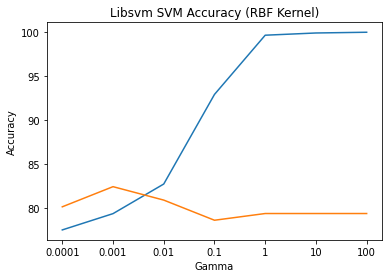
\includegraphics[scale=0.5]{fig/libsvm-acc.png}}
        \subfloat{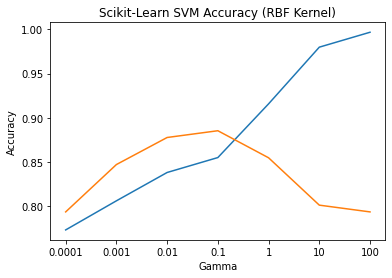
\includegraphics[scale=0.5]{fig/sk-acc.png}}
\end{figure}
In both cases, the training error decreases as $\gamma$ is increased. Since $\gamma$ is inversely related to $\sigma$, this makes sense, as $\gamma$ increasing means that $\sigma$ is decreasing, and by part $(a)$ we know that small $\sigma$ results in a final model that fits the training data more closely.

This can be interpreted as a large $\gamma$ leading to a model that overfits to the training data. Thus when $\gamma$ is small, we have high bias and low variance. The model's decision boundary is too ``smooth'', leading to lower training accuracy but better generalization (and thus better testing accuracy, as exhibited by the training results above).
		

\end{enumerate}

%%%%%%%%%%%%%%%%%%%%
% Perceptron: Theoretical
%%%%%%%%%%%%%%%%%%%%

\section{Perceptron: Theoretical}

\begin{enumerate}
	\item When the algorithm is started with point $\mathbf{x}_1$, it makes 2 mistakes. The two decision boundaries are shown below, with the first (imperfect) decision boundary more transparent than the second (perfect) decision boundary, which is fully opaque.
		\begin{figure}[H]
			\centering
			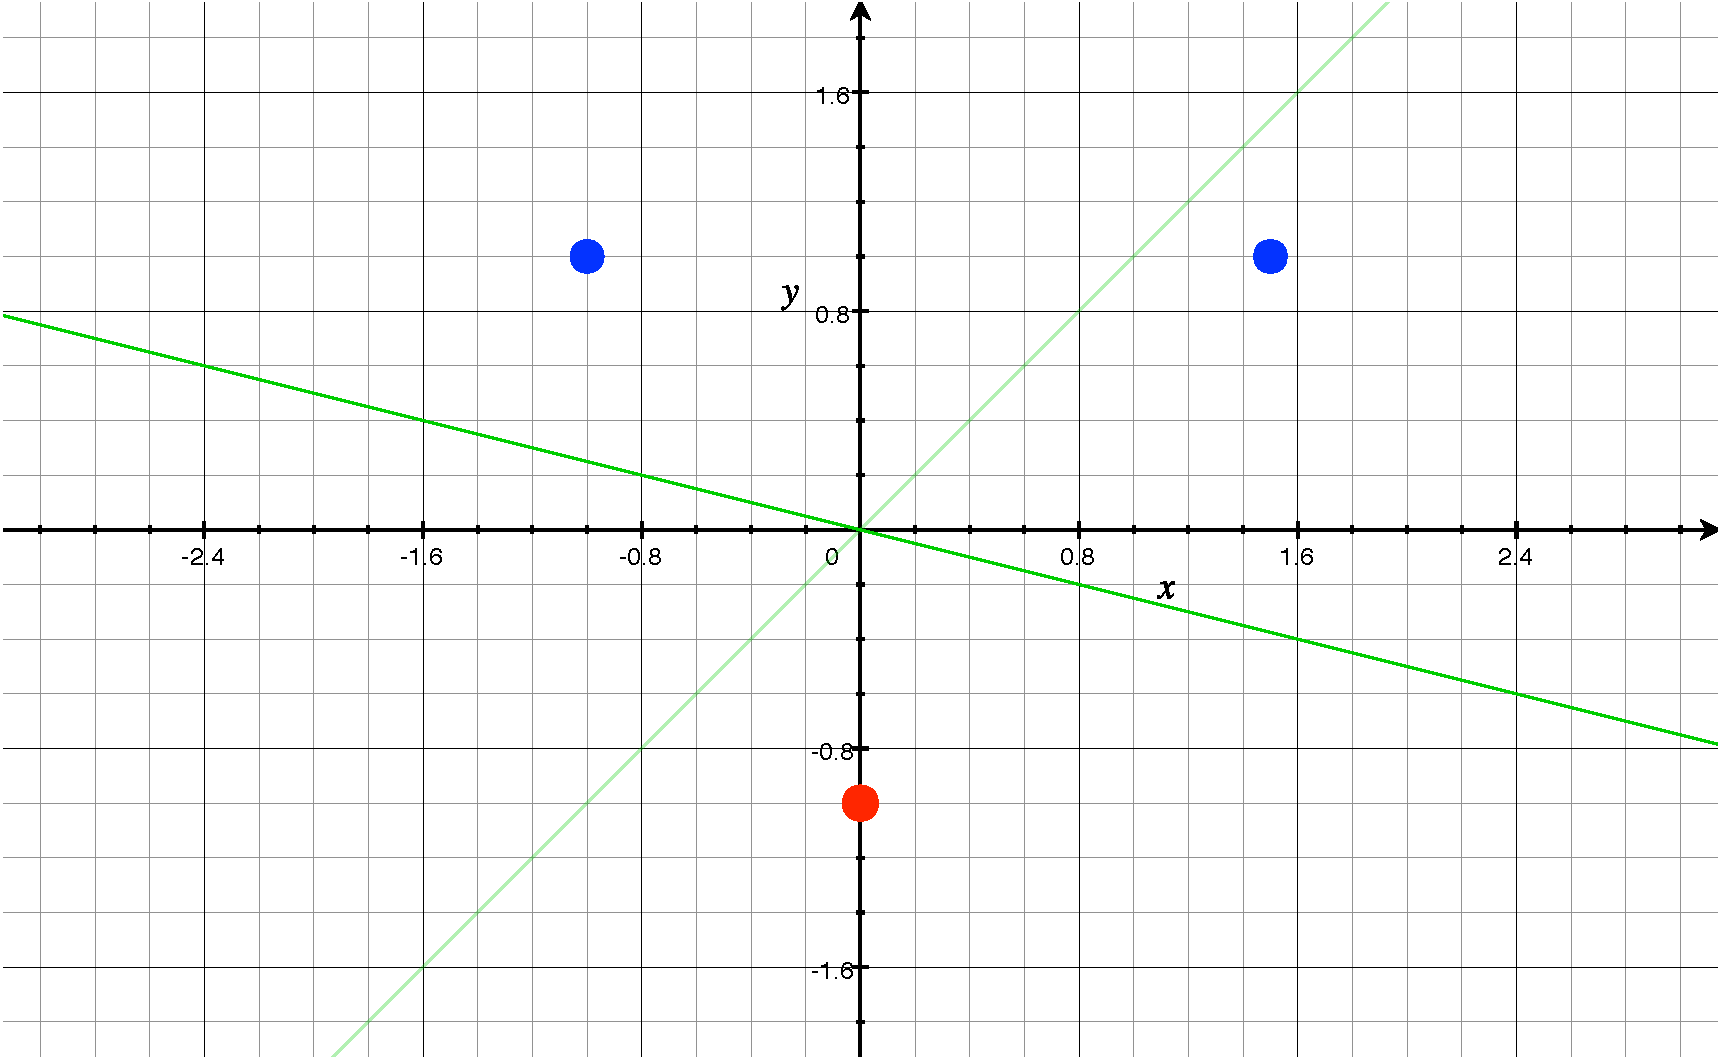
\includegraphics[scale=0.4]{fig/a1.pdf}
			\caption{Perceptron starting with $\mathbf{x}_1$.}
		\end{figure}

		When perceptron starts with $\mathbf{x}_2$, it only makes 1 mistake, i.e. the classifier correctly classifies all three points after the initial correction based on point $\mathbf{x}_2$. The decision boundary for this is shown below.
		\begin{figure}[H]
			\centering
			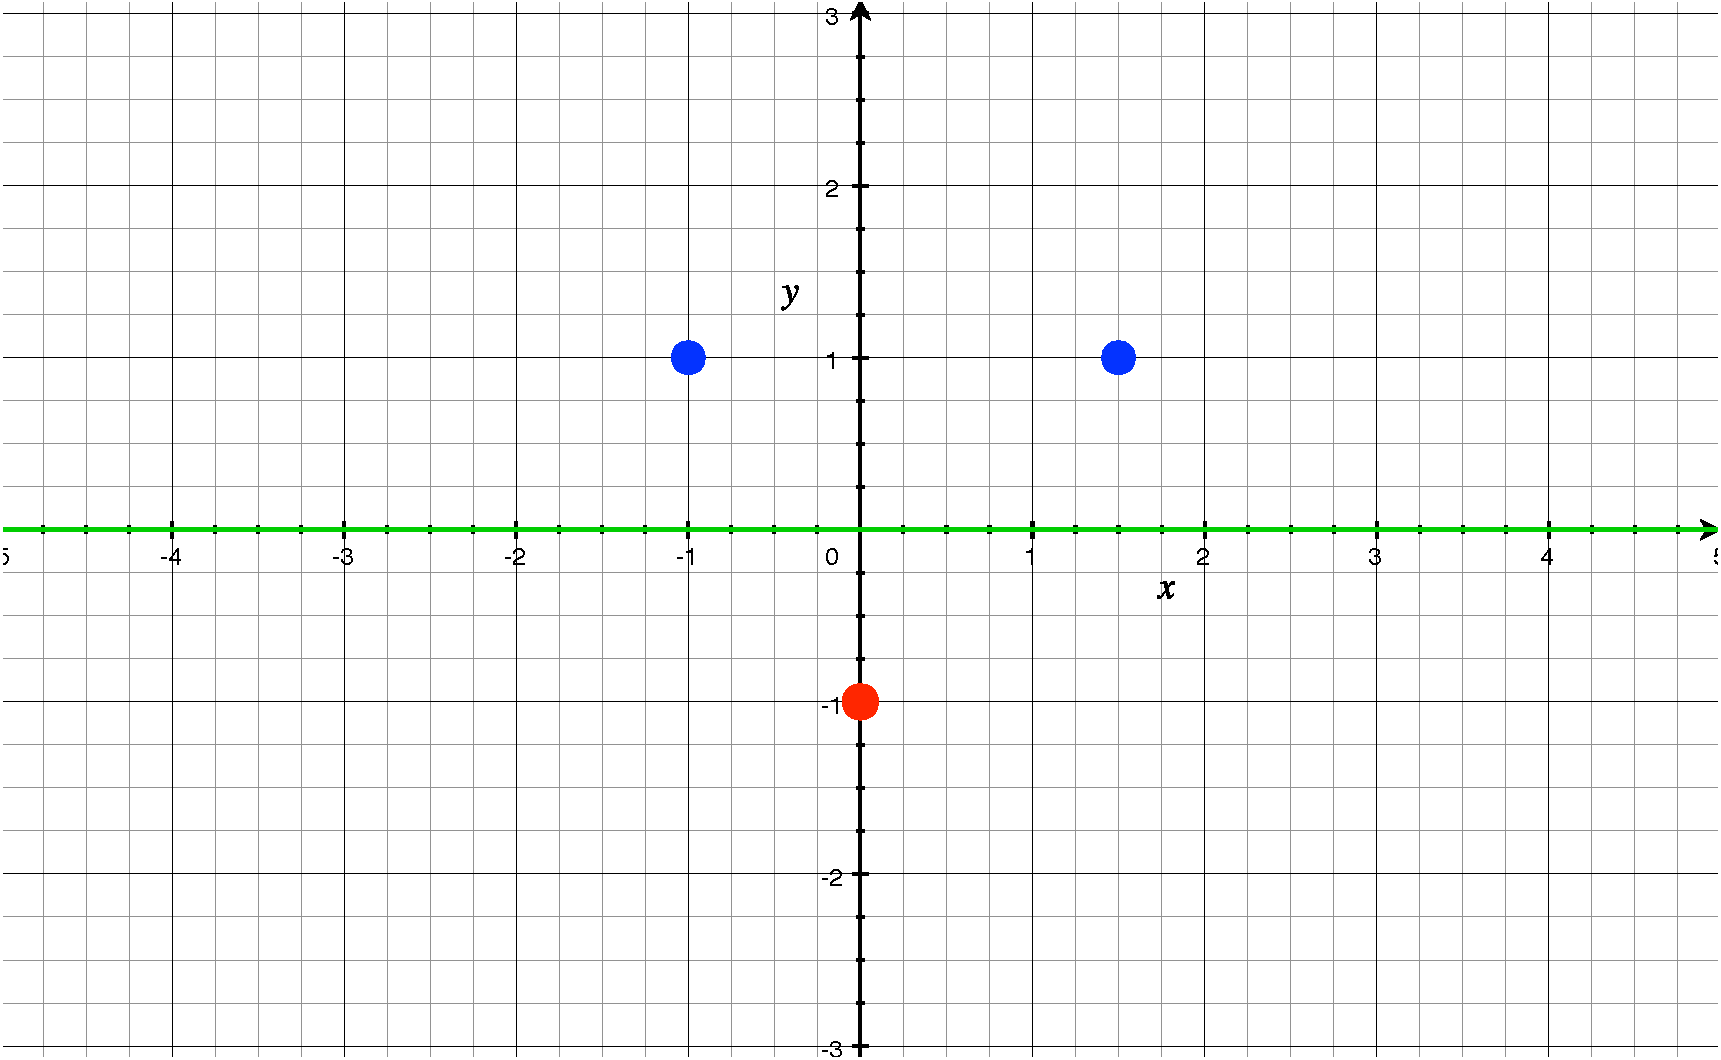
\includegraphics[scale=0.4]{fig/a2.pdf}
			\caption{Perceptron starting with $\mathbf{x}_2$.}
		\end{figure}
		

	\item Starting with $\mathbf{x}_1$, the algorithm makes 6 mistakes as it struggles to correctly classify $\mathbf{x}_1$ after the large change to the decision boundary caused by point $\mathbf{x}_3$. The 6 decision boundaries from this process are shown below, with the oldest decision boundaries the most transparent and the final perfect decision boundary fully opaque.
\begin{figure}[H]
	\centering
	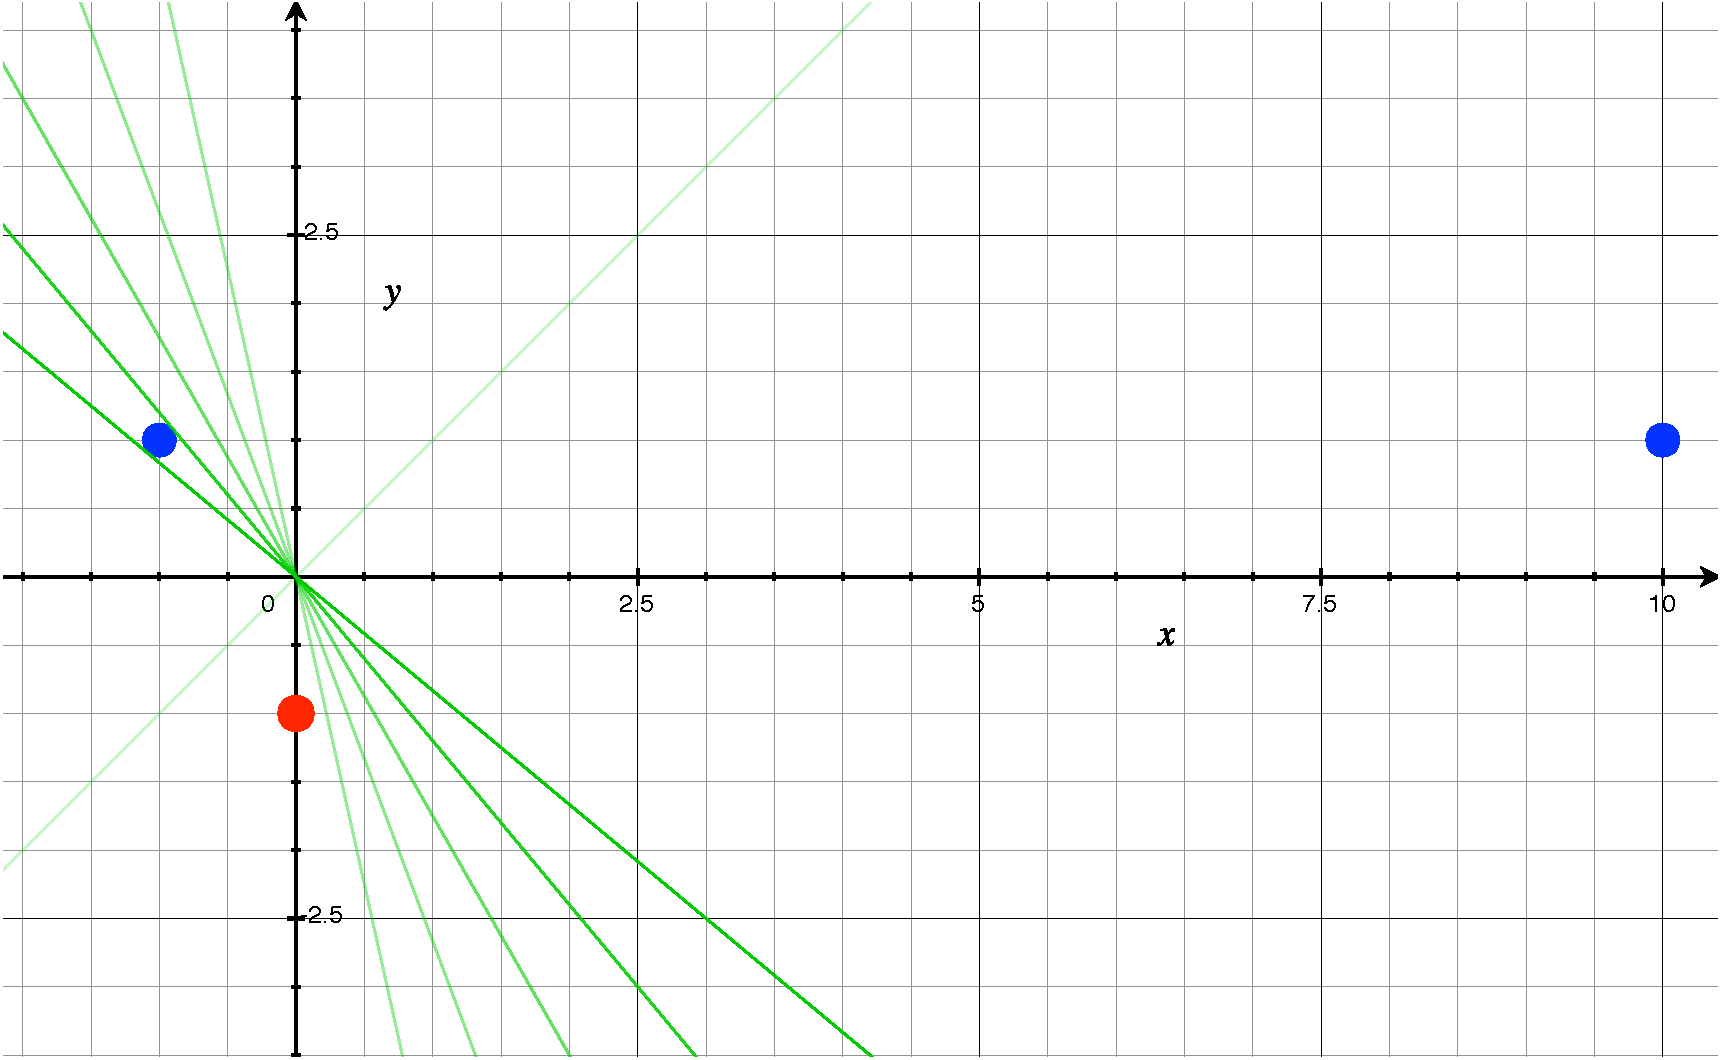
\includegraphics[scale=0.4]{fig/b1.pdf}
	\caption{Perceptron starting with $\mathbf{x}_1$.}
\end{figure}

		When starting with $\mathbf{x}_2$, the algorithm once again only makes 1 mistake and yields the same decision boundary as when starting from $\mathbf{x}_2$ with the original set of points. The decision boundary is shown below.
		\begin{figure}[H]
			\centering
			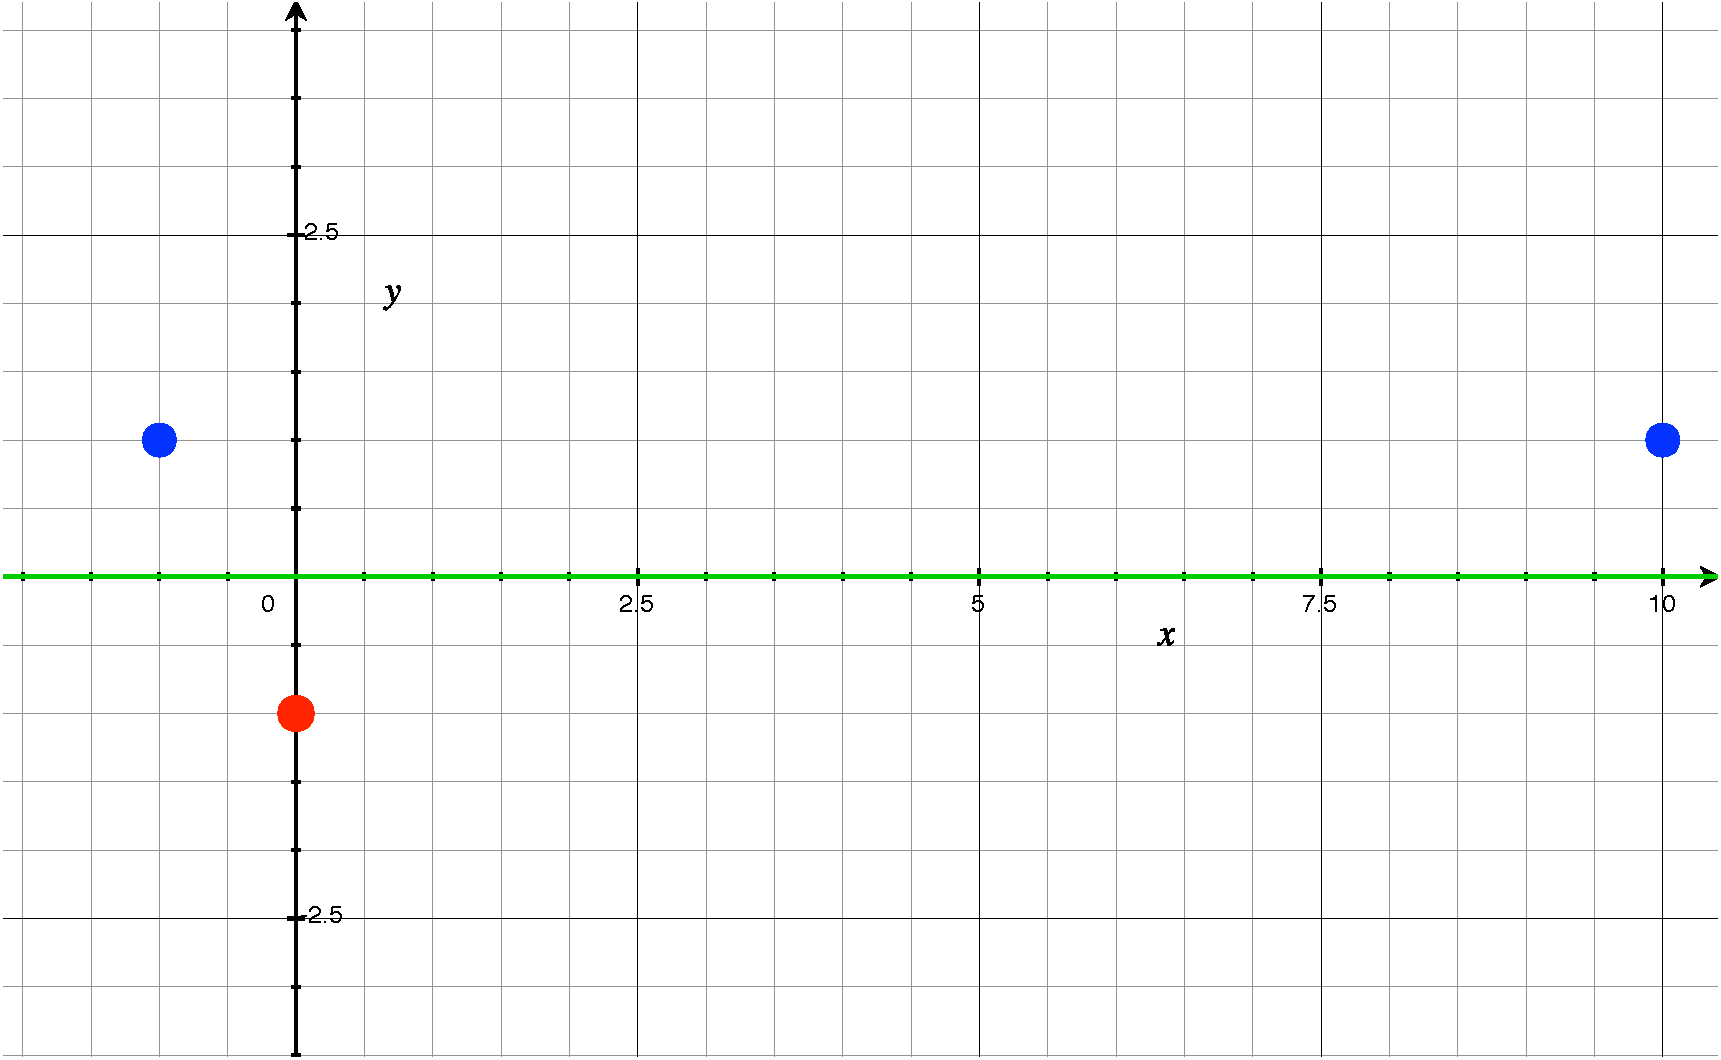
\includegraphics[scale=0.4]{fig/b2.pdf}
			\caption{Perceptron starting with $\mathbf{x}_2$.}
		\end{figure}
		

	\item One possible adversarial procedure, motivated by the negative effect of changing point $\mathbf{x}_2$ in the previous part of the question, would be to sample points that are far away from the final decision boundary.

		Since points close to the boundary are most likely close to other points, we can weight points based on their average distance to other points in the dataset. Points with large average distances should lie on the fringes of the datset, and are thus less likely to lie near the final decision boundary.

		We then sample points according to these weights. Since we are sampling, every point will be seen eventually and thus the algorithm will still converge to a solution.

		More formally, we set the weight $\zeta_i$ for point $\mathbf{x}_i$ to be
		 \[
		\zeta_i = \frac{1}{n} \sum_{j=1}^n \Vert{\mathbf{x}_i - \mathbf{x}_j}\Vert,
		\] then sample point $\mathbf{x}_i$ with probability $\zeta_i / \sum_j \zeta_j$.

		If the separating hyperplane is known beforehand, then we can make this less heuristic by projecting each point $\mathbf{x}_i$ onto the hyperplane and then finding the distance $d_i$ between $\mathbf{x}_i$ and its projection. We then sample points using a similar process, but now the probability of sampling point $\mathbf{x}_i$ is $d_i / \sum_{j} d_j$.
\end{enumerate}



%%%%%%%%%%%%%%%%%%%%
% Perceptron and Balanced Winnow: Programming
%%%%%%%%%%%%%%%%%%%%

\section{Perceptron and Balanced Winnow: Programming}

\textbf{Perceptron:} 
Training curves for the perceptron algorithm with different values of $I$ are plotted below.

\begin{figure}[H]
	\centering
	\subfloat{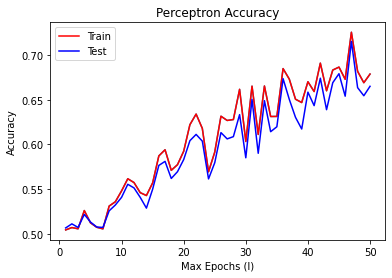
\includegraphics[scale=0.5]{fig/perceptron-50.png}}
	\subfloat{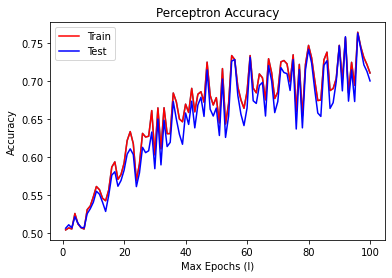
\includegraphics[scale=0.5]{fig/perceptron-100.png}}
\end{figure}
\begin{figure}[H]
	\centering
	\subfloat{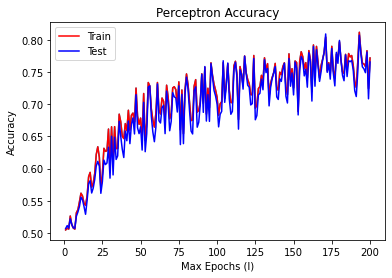
\includegraphics[scale=0.5]{fig/perceptron-200.png}}
\end{figure}
The algorithm seems to quickly improve both its training and testing error at first, and the improvement rate decreases the longer the algorithm runs. Notably, the testing error very closely matches the training error. It consistenly is just slightly below the training error, regardless of how long the algorithm is run.

The trend in this data is straightforward, so increasing the maximum number of epochs should result in training curves that follow this same trend (we expect further improvement, but the amount of improvement per extra epoch is expected to decrease).

\textbf{Balanced Winnow:} 
Training curves for the balanced winnow algorithm with $\eta = 0.1$ and different values of $I$ are plotted below.

\begin{figure}[H]
        \centering
	\subfloat{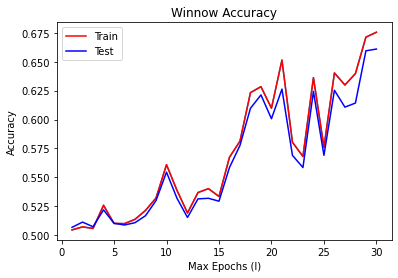
\includegraphics[scale=0.5]{fig/winnow-30.png}}
	\subfloat{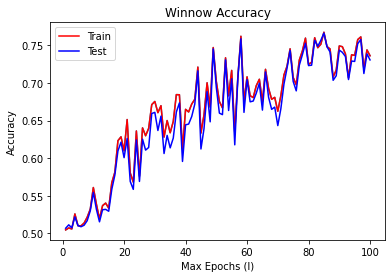
\includegraphics[scale=0.5]{fig/winnow-100.png}}
\end{figure}
\begin{figure}[H]
        \centering
        \subfloat{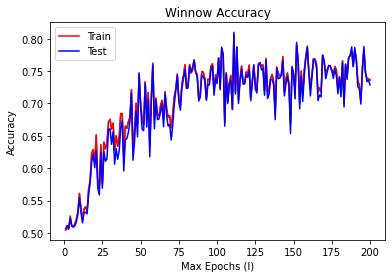
\includegraphics[scale=0.5]{fig/winnow-200.png}}
\end{figure}

This exists behavior similar to that of the perceptron algorithm, with much improvement initially that slows down in further epochs, as well as testing error that is consistenly just slightly less than the training error. By epoch 100, the algorithm seems to have reached a stable state around 75\% training and testing accuracy.


\end{document}
